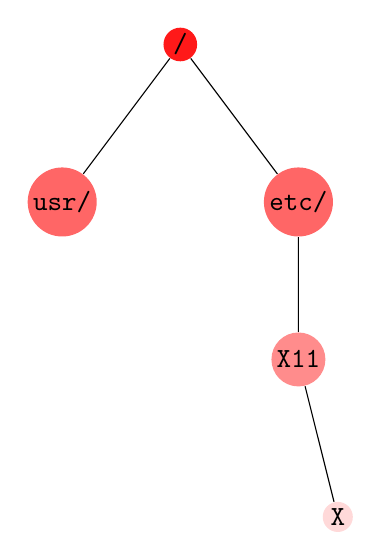
\begin{tikzpicture}[level distance=20mm] 
  \tikzstyle{every node}=[fill=red!90,circle,inner sep=1pt] 
  \tikzstyle{level 1}=[sibling distance=30mm, 
  set style={{every node}+=[fill=red!60]}] 
  \tikzstyle{level 2}=[sibling distance=20mm,
  set style={{every node}+=[fill=red!45]}] 
  \tikzstyle{level 3}=[sibling distance=10mm,
  set style={{every node}+=[fill=red!15]}]
  
  \node {\texttt{/}} 
    child {node {\texttt{usr/}}
    } 
    child {node {\texttt{etc/}} 
      child {node {\texttt{X11}} 
        child[fill=none] 
        {edge from parent[draw=none]}
        child {node {\texttt{X}}} 
      }
    };
\end{tikzpicture}
